\documentclass[onesided]{article}\usepackage[]{graphicx}\usepackage[]{color}
% maxwidth is the original width if it is less than linewidth
% otherwise use linewidth (to make sure the graphics do not exceed the margin)
\makeatletter
\def\maxwidth{ %
  \ifdim\Gin@nat@width>\linewidth
    \linewidth
  \else
    \Gin@nat@width
  \fi
}
\makeatother

\definecolor{fgcolor}{rgb}{0.345, 0.345, 0.345}
\newcommand{\hlnum}[1]{\textcolor[rgb]{0.686,0.059,0.569}{#1}}%
\newcommand{\hlstr}[1]{\textcolor[rgb]{0.192,0.494,0.8}{#1}}%
\newcommand{\hlcom}[1]{\textcolor[rgb]{0.678,0.584,0.686}{\textit{#1}}}%
\newcommand{\hlopt}[1]{\textcolor[rgb]{0,0,0}{#1}}%
\newcommand{\hlstd}[1]{\textcolor[rgb]{0.345,0.345,0.345}{#1}}%
\newcommand{\hlkwa}[1]{\textcolor[rgb]{0.161,0.373,0.58}{\textbf{#1}}}%
\newcommand{\hlkwb}[1]{\textcolor[rgb]{0.69,0.353,0.396}{#1}}%
\newcommand{\hlkwc}[1]{\textcolor[rgb]{0.333,0.667,0.333}{#1}}%
\newcommand{\hlkwd}[1]{\textcolor[rgb]{0.737,0.353,0.396}{\textbf{#1}}}%
\let\hlipl\hlkwb

\usepackage{framed}
\makeatletter
\newenvironment{kframe}{%
 \def\at@end@of@kframe{}%
 \ifinner\ifhmode%
  \def\at@end@of@kframe{\end{minipage}}%
  \begin{minipage}{\columnwidth}%
 \fi\fi%
 \def\FrameCommand##1{\hskip\@totalleftmargin \hskip-\fboxsep
 \colorbox{shadecolor}{##1}\hskip-\fboxsep
     % There is no \\@totalrightmargin, so:
     \hskip-\linewidth \hskip-\@totalleftmargin \hskip\columnwidth}%
 \MakeFramed {\advance\hsize-\width
   \@totalleftmargin\z@ \linewidth\hsize
   \@setminipage}}%
 {\par\unskip\endMakeFramed%
 \at@end@of@kframe}
\makeatother

\definecolor{shadecolor}{rgb}{.97, .97, .97}
\definecolor{messagecolor}{rgb}{0, 0, 0}
\definecolor{warningcolor}{rgb}{1, 0, 1}
\definecolor{errorcolor}{rgb}{1, 0, 0}
\newenvironment{knitrout}{}{} % an empty environment to be redefined in TeX

\usepackage{alltt}
\usepackage[T1]{fontenc}
\linespread{1.5} % Line spacing - Palatino needs more space between lines
\usepackage{microtype} % Slightly tweak font spacing for aesthetics

\usepackage[hmarginratio=1:1,columnsep=20pt]{geometry} % Document margins
%\usepackage{multicol} % Used for the two-column layout of the document
\usepackage[hang, small,labelfont=bf,up,textfont=it,up]{caption} % Custom captions under/above floats in tables or figures
\usepackage{booktabs} % Horizontal rules in tables
\usepackage{float} % Required for tables and figures in the multi-column environment - they need to be placed in specific locations with the [H] (e.g. \begin{table}[H])

\usepackage{lettrine} % The lettrine is the first enlarged letter at the beginning of the text
\usepackage{paralist} % Used for the compactitem environment which makes bullet points with less space between them

% to ignore texts: good for thank messages and paper submissions.
      % \fbox{\phantom{This text will be invisible too, but a box will be printed arround it.}}

\usepackage{abstract} % Allows abstract customization
\renewcommand{\abstractnamefont}{\normalfont\bfseries} % Set the "Abstract" text to bold
%\renewcommand{\abstracttextfont}{\normalfont\small\itshape} % Set the abstract itself to small italic text

\usepackage[]{titlesec} % Allows customization of titles
\renewcommand\thesection{\Roman{section}} % Roman numerals for the sections
\renewcommand\thesubsection{\Roman{subsection}} % Roman numerals for subsections
\titleformat{\section}[block]{\large\scshape\centering}{\thesection.}{1em}{} % Change the look of the section titles
\titleformat{\subsection}[block]{\large}{\thesubsection.}{1em}{} % Change the look of the section titles

\usepackage{fancybox, fancyvrb, calc}
\usepackage[svgnames]{xcolor}
\usepackage{epigraph}
\usepackage{longtable}
\usepackage{pdflscape}
\usepackage{graphics}
\usepackage{pbox} % \pbox{20cm}{This is the first \\ cell}
\usepackage{amsfonts}
\usepackage{amsmath}
\usepackage{amssymb}
\usepackage{rotating}
\usepackage{paracol}
\usepackage{textcomp}
\usepackage[export]{adjustbox}
\usepackage{afterpage}
\usepackage{filecontents}
\usepackage{color}
\usepackage{latexsym}
\usepackage{lscape}       %\begin{landscape} and \end{landscape}
\usepackage{wasysym}
\usepackage{dashrule}

\usepackage{framed}
\usepackage{tree-dvips}
\usepackage{pgffor}
\usepackage[]{authblk}
\usepackage{setspace}
\usepackage{array}
\usepackage[latin1]{inputenc}
\usepackage{hyperref}     %desactivar para link rojos
\usepackage{graphicx}
\usepackage{dcolumn} % for R tables
\usepackage{multirow} % For multirow in tables
\usepackage{pifont}
\usepackage{listings}




% hypothesis / theorem package begin
\usepackage{amsthm}
\usepackage{thmtools}
\declaretheoremstyle[
spaceabove=6pt, spacebelow=6pt,
headfont=\normalfont\bfseries,
notefont=\mdseries, notebraces={(}{)},
bodyfont=\normalfont,
postheadspace=0.6em,
headpunct=:
]{mystyle}
\declaretheorem[style=mystyle, name=Hypothesis, preheadhook={\renewcommand{\thehyp}{H\textsubscript{\arabic{hyp}}}}]{hyp}

\usepackage{cleveref}
\crefname{hyp}{hypothesis}{hypotheses}
\Crefname{hyp}{Hypothesis}{Hypotheses}
% hypothesis / theorem package end


%----------------------------------------------------------------------------------------
% Other ADDS-ON
%----------------------------------------------------------------------------------------

% independence symbol \independent
\newcommand\independent{\protect\mathpalette{\protect\independenT}{\perp}}
\def\independenT#1#2{\mathrel{\rlap{$#1#2$}\mkern2mu{#1#2}}}







\hypersetup{
    bookmarks=true,         % show bookmarks bar?
    unicode=false,          % non-Latin characters in Acrobat's bookmarks
    pdftoolbar=true,        % show Acrobat's toolbar?
    pdfmenubar=true,        % show Acrobat's menu?
    pdffitwindow=true,     % window fit to page when opened
    pdfstartview={FitH},    % fits the width of the page to the window
    pdftitle={My title},    % title
    pdfauthor={Author},     % author
    pdfsubject={Subject},   % subject of the document
    pdfcreator={Creator},   % creator of the document
    pdfproducer={Producer}, % producer of the document
    pdfkeywords={keyword1} {key2} {key3}, % list of keywords
    pdfnewwindow=true,      % links in new window
    colorlinks=true,       % false: boxed links; true: colored links
    linkcolor=ForestGreen,          % color of internal links (change box color with linkbordercolor)
    citecolor=ForestGreen,        % color of links to bibliography
    filecolor=ForestGreen,      % color of file links
    urlcolor=ForestGreen           % color of external links
}

%\usepackage[nodayofweek,level]{datetime} % to have date within text

\newcommand{\LETT}[3][]{\lettrine[lines=4,loversize=.2,#1]{\smash{#2}}{#3}} % letrine customization



% comments on margin
  % Select what to do with todonotes: 
  % \usepackage[disable]{todonotes} % notes not showed
  \usepackage[draft]{todonotes}   % notes showed
  % usage: \todo{This is a note at margin}

\usepackage{cooltooltips}

%%% bib begin
\usepackage[american]{babel}
\usepackage{csquotes}
\usepackage[backend=biber,style=authoryear,dashed=false,doi=false,isbn=false,url=false,arxiv=false]{biblatex}
%\DeclareLanguageMapping{american}{american-apa}
\addbibresource{/Users/hectorbahamonde/Bibliografia_PoliSci/library.bib} 
\addbibresource{/Users/hectorbahamonde/Bibliografia_PoliSci/Bahamonde_BibTex2013.bib} 

% USAGES
%% use \textcite to cite normal
%% \parencite to cite in parentheses
%% \footcite to cite in footnote
%% the default can be modified in autocite=FOO, footnote, for ex. 
%%% bib end

\usepackage{fancyhdr} % Headers and footers
\pagestyle{fancy} % All pages have headers and footers
\fancyhead{} % Blank out the default header
\fancyfoot{} % Blank out the default footer
\fancyhead[C]{Regression Discontinuity Designs: Fuzzy} % Custom header text
\fancyfoot[RO,LE]{\thepage} % Custom footer text
\IfFileExists{upquote.sty}{\usepackage{upquote}}{}
\begin{document}
% DOCUMENT ID
%----------------------------------------------------------------------------------------
%	CONTENT
%----------------------------------------------------------------------------------------

%\graphicspath{
%{/Users/hectorbahamonde/RU/Term5/Experiments_Redlawsk/Experiment/Data/}
%}



%%%%%%%%%%%%%%%%%%%%%%%%%%%%%%%%%%%%%%%%%%%%%%
% begin knitr stuff


%%%%%%%%%%%%%%%%%%%%%%%%%%%%%%%%%%%%%%%%%%%%%%





\hspace{-5mm}{\bf Profesor}: H\'ector Bahamonde, PhD.\\
\texttt{e:}\href{mailto:hector.bahamonde@uoh.cl}{\texttt{hector.bahamonde@uoh.cl}}\\
\texttt{w:}\href{http://www.hectorbahamonde.com}{\texttt{www.hectorbahamonde.com}}\\
{\bf Curso}: MLE.\\
\hspace{-5mm}{\bf TA}: Gonzalo Barr\'ia.


\section*{Regression Discontinuity Designs (RDDs)---Fuzzy Designs}

Motivemos el modelo RDD general:

\begin{equation}\label{eq:1}
y_{i} \;=\; \beta_{0} + \beta_{1}x_{i} + \pi z_{i} + \rho x_{i}z_{i} + \epsilon_{i}
\end{equation}

En los dise\~nos RDD \emph{sharp} existe una relaci\'on \emph{determinista} en c\'omo $z$ clasifica a $x$ \parencite[202]{Hahn2001a}:


\begin{center}
$z_{i} = \left \{ 
\begin{matrix}\label{det:1}
     1 & \text{si} \; x \le \text{corte} \\
     0 & \text{si} \; x > \text{corte}

\end{matrix}\right. $
\end{center}

Ya sabemos que el corte no es aleatorio. Pero en los dise\~nos \emph{fuzzy} $z$ no es determinista, si no que hay variables adicionales que son anteriores a $z$ que operan en la clasificaci\'on de $x$. 

\paragraph{El problema}El problema substantivo detr\'as del $z$ en un \emph{fuzzy design} es que hay un problema de ``\emph{compliance}'': no todos los sujetos involucrados en el dise\~no ``cumplen'' con su r\'egimen experimental esperado. Por ejemplo, los sujetos que debieran haber tomado el tratamiento, no lo hicieron (el experimento sali\'o mal!). O tambi\'en, el experimentador no ten\'ia las herramientas para ``forzar'' la clasificaci\'on experimental. 

\paragraph{Ejemplo 1}Imag\'inate que estudiando campa\~nas pol\'iticas env\'ias por carta un tr\'iptico con informaci\'on sobre una campa\~na. Despu\'es, la idea es llamar por tel\'efono a hogares de control (sin tr\'iptico) y tratamiento (con tr\'iptico) y hacerles una encuesta. \emph{Qu\'e pasa si aquellos que debieran haber sido tratados no leyeron el tr\'iptico?} Esas personas debieran haber sido ``tratadas'', pero dado que no leyeron el folleto, ahora est\'an en el r\'egimen de control. Aqu\'i el experimentador no puede forzar la lectura del folleto. 

\paragraph{Ejemplo 2}Otro tipo de dise\~nos fuzzy \emph{no} tiene que ver con errores en el proceso de dise\~no experimental. Por ejemplo, \textcite[244]{ErikMe2014} se interes\'o en si el grado en que los partidos pol\'iticos isl\'amicos afectaba el empoderamiento femenino. Aqu\'i el eje $x$ es el margen por el que los partidos isl\'amicos ganan las elecciones, y el eje $y$ es la participaci\'on de mujeres que asiste al colegio. En este caso es f\'acil ver que existir\'a un \emph{overlap} entre las observaciones, no existiendo una clasificaci\'on determinista entre quienes recibe el ``tratamiento'' y quienes no.

Entonces, \emph{fuzzy} va m\'as all\'a de errores en la administraci\'on del tratamiento.

\paragraph{Soluci\'on} Existen dos maneras de analizar este tipo de datos:

\begin{enumerate}
  \item Instrumental Variables y 2SLS.
  \item Regresi\'on Lineal Local (``\emph{local linear regression}'').
\end{enumerate}

\section{Estimador}

En los dise\~nos \emph{sharp} trabajamos con el ATE o ATT. Sin embargo, en los dise\~nos \emph{fuzzy} no existe ``\emph{perfect compliance}''. Es por esto que debemos trabajar con otro estimador, el \emph{Intention-to-treat effects} o \emph{ITT}. Este estimador no se concentra en quien recibi\'o el tratamiento, sino en quien nosotros ``\emph{intent\'abamos}'' tratar.

El ITT es m\'as sencillo y realista. En general se entiende que el \emph{ITT} es la diferencia entre los sujetos $y_{1}$ bajo r\'egimen de tratamiento $z(1)$ y los sujetos $y_{0}$ bajo r\'egimen de control $z(0)$, independiente de problemas ``\emph{compliance}'' y otros posibles problemas que puedan existir. Al obviar todas las posibles alternativas que podr\'ian haber salido mal (\emph{compliance}, por ej.), el \emph{ITT} mide la \emph{elegibilidad} al tratamiento ($z_{1}$), independiente de si se trata de $y_{1}$ o $y_{0}$.

%https://www.ncbi.nlm.nih.gov/pmc/articles/PMC3159210/?report=reader

\section{Instrumental Variables y 2SLS}

Dado que $z$ asigna 0's o 1's con cierta \emph{probabilidad} (i.e. no \emph{deterministamente}), el ``no-cumplimiento'' es posible de ser modelado. De hecho, \textcite[]{Hahn2001a} demuestran que $z$ puede ser estimado de la misma manera que una {\bf variable instrumental} v\'ia a \emph{two-stage least square design} (2SLS). 

La manera en que hacemos esto es que estimamos $z$ como funci\'on de $x$ en la primera etapa. Despu\'es, se obtiene $\hat z$. En la segunda etapa se estima $y$ como funci\'on de $x$ y $\hat z$.

Es decir, en la primera etapa se estima \autoref{et:1}

\begin{equation}\label{et:1}
z_{i} \;=\; \beta_{0} + \beta_{1}x_{i} + \epsilon_{i}
\end{equation}

y en la segunda etapa se estima \autoref{et:2}

\begin{equation}\label{et:2}
y_{i} \;=\; \beta_{0} + \beta_{1}x_{i} + \pi \hat z_{i} + \epsilon_{i}
\end{equation}


Cocinemos unos datos. En esta parte usaremos el paquete \texttt{rddtools} que se encarga de estimar el modelo v\'ia 2SLS.

\begin{knitrout}
\definecolor{shadecolor}{rgb}{0.969, 0.969, 0.969}\color{fgcolor}\begin{kframe}
\begin{alltt}
\hlstd{mu} \hlkwb{<-} \hlkwd{c}\hlstd{(}\hlnum{0}\hlstd{,} \hlnum{0}\hlstd{)} \hlcom{# los promedios de ambos vectores}
\hlstd{sigma} \hlkwb{<-} \hlkwd{matrix}\hlstd{(}\hlkwd{c}\hlstd{(}\hlnum{1}\hlstd{,} \hlnum{0.7}\hlstd{,} \hlnum{0.7}\hlstd{,} \hlnum{1}\hlstd{),} \hlkwc{ncol} \hlstd{=} \hlnum{2}\hlstd{)} \hlcom{# una matriz de varianza-covarianza}
\hlkwd{p_load}\hlstd{(MASS)}
\hlstd{d} \hlkwb{<-} \hlkwd{as.data.frame}\hlstd{(}\hlkwd{mvrnorm}\hlstd{(}\hlnum{2000}\hlstd{, mu, sigma))} \hlcom{# creamos la base de datos}
\hlkwd{colnames}\hlstd{(d)} \hlkwb{<-} \hlkwd{c}\hlstd{(}\hlstr{"x"}\hlstd{,} \hlstr{"y"}\hlstd{)} \hlcom{# le cambiamos los nombres}
\hlstd{corte} \hlkwb{=} \hlnum{0} \hlcom{# definir el corte}
\hlstd{d}\hlopt{$}\hlstd{z} \hlkwb{<-} \hlkwd{ifelse}\hlstd{(d}\hlopt{$}\hlstd{x} \hlopt{<}  \hlstd{corte,} \hlnum{0}\hlstd{,} \hlnum{0.8}\hlstd{)} \hlcom{# introducimos FUZZYNESS }
\hlcom{# Si d$x < corte, z es 0 con un 100% de probabilidad.}
\hlcom{# Si d$x > corte, z es 1 con un 80% de probabilidad. }
\hlcom{# "Compliance"!}
\end{alltt}
\end{kframe}
\end{knitrout}

Aqu\'i hemos cocinado datos multivariados usando la funci\'on \texttt{mvrnorm} (\emph{multivariate random normal}). Como es multivariada, tendremos m\'as de un vector (en este caso dos). 

Hasta ahora \texttt{d\$z} es un vector de probabilidades (0, y .8). 

\begin{knitrout}
\definecolor{shadecolor}{rgb}{0.969, 0.969, 0.969}\color{fgcolor}\begin{kframe}
\begin{alltt}
\hlkwd{table}\hlstd{(d}\hlopt{$}\hlstd{z)}
\end{alltt}
\begin{verbatim}
## 
##    0  0.8 
##  990 1010
\end{verbatim}
\end{kframe}
\end{knitrout}

Metamos ese vector de probabilidades en una funci\'on para convertirlos en 0's y 1's

\begin{knitrout}
\definecolor{shadecolor}{rgb}{0.969, 0.969, 0.969}\color{fgcolor}\begin{kframe}
\begin{alltt}
\hlstd{d}\hlopt{$}\hlstd{z} \hlkwb{<-} \hlkwd{sapply}\hlstd{(}\hlkwc{X} \hlstd{= d}\hlopt{$}\hlstd{z,} \hlkwc{FUN} \hlstd{=} \hlkwa{function}\hlstd{(}\hlkwc{x}\hlstd{)} \hlkwd{rbinom}\hlstd{(}\hlnum{1}\hlstd{,} \hlnum{1}\hlstd{,} \hlkwc{prob} \hlstd{= x))} \hlcom{# funcion}
\end{alltt}
\end{kframe}
\end{knitrout}

Ve\'amos c\'omo qued\'o:

\begin{knitrout}
\definecolor{shadecolor}{rgb}{0.969, 0.969, 0.969}\color{fgcolor}\begin{kframe}
\begin{alltt}
\hlkwd{table}\hlstd{(d}\hlopt{$}\hlstd{z)}
\end{alltt}
\begin{verbatim}
## 
##    0    1 
## 1177  823
\end{verbatim}
\end{kframe}
\end{knitrout}

Ahora fabriquemos el efecto de $z$ en $y$, y digamos que es $2$ (combinaci\'on lineal).

\begin{knitrout}
\definecolor{shadecolor}{rgb}{0.969, 0.969, 0.969}\color{fgcolor}\begin{kframe}
\begin{alltt}
\hlstd{d}\hlopt{$}\hlstd{y} \hlkwb{<-} \hlstd{d}\hlopt{$}\hlstd{y} \hlopt{+} \hlstd{d}\hlopt{$}\hlstd{z} \hlopt{*} \hlnum{2}
\end{alltt}
\end{kframe}
\end{knitrout}

Ahora grafiqu\'emos

\begin{knitrout}
\definecolor{shadecolor}{rgb}{0.969, 0.969, 0.969}\color{fgcolor}\begin{kframe}
\begin{alltt}
\hlkwd{plot}\hlstd{(d}\hlopt{$}\hlstd{x, d}\hlopt{$}\hlstd{y,}
     \hlkwc{col} \hlstd{=} \hlkwd{c}\hlstd{(}\hlstr{"steelblue"}\hlstd{,} \hlstr{"darkred"}\hlstd{)[}\hlkwd{factor}\hlstd{(d}\hlopt{$}\hlstd{z)],}  \hlcom{# asignar color para z(1) y z(0)}
     \hlkwc{pch}\hlstd{=} \hlnum{20}\hlstd{,} \hlcom{# geometria de los circulos}
     \hlkwc{cex} \hlstd{=} \hlnum{0.5}\hlstd{,} \hlcom{# tamano de los circulos}
     \hlkwc{xlab} \hlstd{=} \hlstr{"x"}\hlstd{,}
     \hlkwc{ylab} \hlstd{=} \hlstr{"y"}\hlstd{)}
\hlcom{# linea vertical }
\hlkwd{abline}\hlstd{(}\hlkwc{v} \hlstd{=} \hlnum{0}\hlstd{,} \hlkwc{lty} \hlstd{=} \hlnum{2}\hlstd{)}
\end{alltt}
\end{kframe}

{\centering 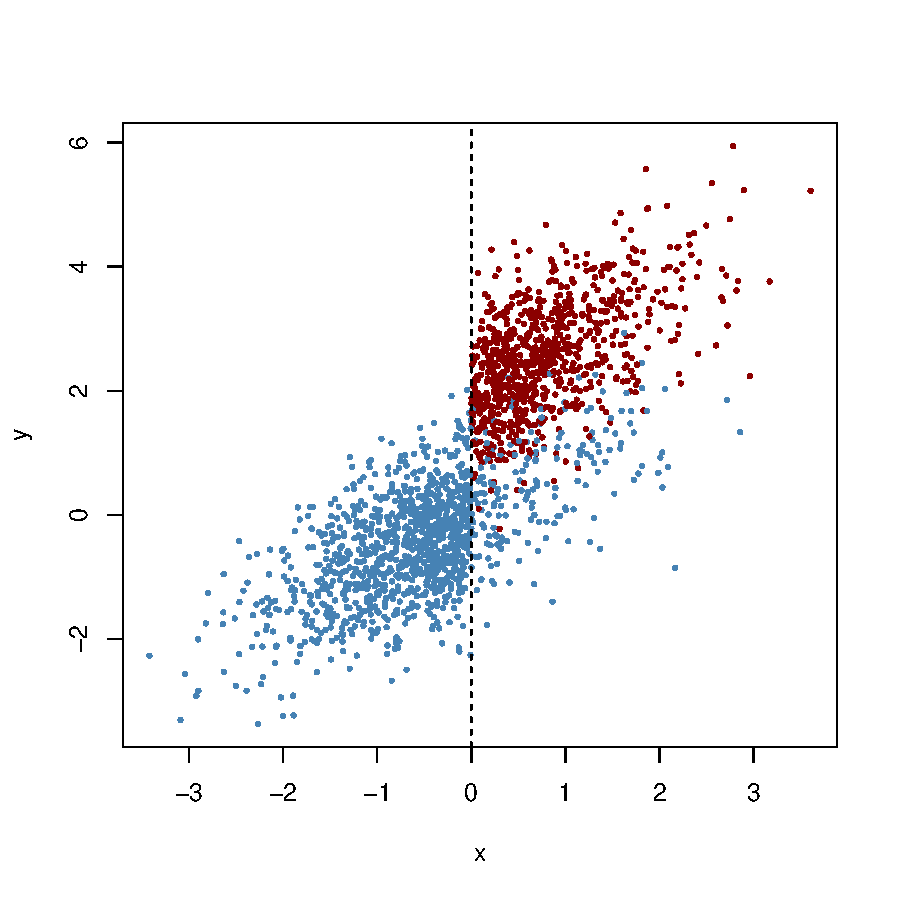
\includegraphics[width=\maxwidth]{figure/chunk:6-1} 

}



\end{knitrout}

Ahora que tenemos los datos listos, estimemos el modelo.

\begin{knitrout}
\definecolor{shadecolor}{rgb}{0.969, 0.969, 0.969}\color{fgcolor}\begin{kframe}
\begin{alltt}
\hlcom{# Estimar Fuzzy RDD}
\hlkwd{p_load}\hlstd{(rddtools)}
\hlcom{# declarar que objeto "d" es un data frame de RDD}
\hlstd{data} \hlkwb{<-} \hlkwd{rdd_data}\hlstd{(d}\hlopt{$}\hlstd{y, d}\hlopt{$}\hlstd{x,}
                 \hlkwc{cutpoint} \hlstd{= corte,}
                 \hlkwc{z} \hlstd{= d}\hlopt{$}\hlstd{z}
                 \hlstd{)}
\hlcom{# veamos}
\hlkwd{head}\hlstd{(data)}
\end{alltt}
\begin{verbatim}
##            x         y z
## 1  0.7605976  1.934505 1
## 2  0.3326682  2.223360 1
## 3 -1.1249196 -0.899735 0
## 4 -1.4135165 -0.670849 0
## 5 -2.6293837 -2.527171 0
## 6  1.2715528  2.057119 1
\end{verbatim}
\begin{alltt}
\hlcom{# Estimar modelo fuzzy RDD}
\hlkwd{rdd_reg_lm}\hlstd{(}\hlkwc{rdd_object} \hlstd{= data,} \hlkwc{slope} \hlstd{=} \hlstr{"same"}\hlstd{)}
\end{alltt}
\begin{verbatim}
## ### RDD regression: parametric ###
## 	Polynomial order:  1 
## 	Slopes:  same 
## 	Number of obs: 2000 (left: 990, right: 1010)
## 
## 	Coefficient:
##   Estimate Std. Error t value              Pr(>|t|)    
## D 1.905460   0.067511  28.224 < 0.00000000000000022 ***
## ---
## Signif. codes:  0 '***' 0.001 '**' 0.01 '*' 0.05 '.' 0.1 ' ' 1
\end{verbatim}
\begin{alltt}
\hlcom{# En este caso, D es el efecto causal, o rho. Es aprox. 2. }
\end{alltt}
\end{kframe}
\end{knitrout}


\section{\emph{Local Linear Regression}}

Otra manera de estimar es estimando un modelo justo en el corte. Este es un enfoque que usa s\'olo las observaciones cerca del corte---i.e. una regresi\'on \emph{local}---en una especie de ``mini regresi\'on''. 

\begin{itemize}
	\item El problema es que perdemos poder estadistico ({\color{red}?}).
	\item El supuesto es que las observaciones que rodean el corte son muy similares en cuanto a sus valores de $x$. {\color{red}Por que es esto importante?} En base a este supuesto se construye el \emph{contrafactual}. 
\end{itemize}

Si quisi\'eramos estimar una regresi\'on local, la primera pregunta ser\'ia cu\'an ancho o delgado es nuestro ``ancho de banda'' (o ``\emph{bandwidth}''). Afortunadamente \textcite{Imbens2012} desarrollaron un estimador que encuentra el ``ancho de banda'' m\'as \'optimo al rededor del corte. Ellos demuestran que usando s\'olo esas observaciones al rededor del corte se minimizan los errores cuadrados del (``mini'') modelo. Este estimador est\'a contenido en la funci\'on \texttt{IKbandwidth} del paquete \texttt{rdd}. 

\begin{knitrout}
\definecolor{shadecolor}{rgb}{0.969, 0.969, 0.969}\color{fgcolor}\begin{kframe}
\begin{alltt}
\hlkwd{p_load}\hlstd{(rdd)}
\hlstd{band} \hlkwb{<-} \hlkwd{IKbandwidth}\hlstd{(d}\hlopt{$}\hlstd{x, d}\hlopt{$}\hlstd{y)}
\hlstd{band} \hlcom{# ancho de banda optimo}
\end{alltt}
\begin{verbatim}
## [1] 0.4034962
\end{verbatim}
\begin{alltt}
\hlcom{# corta la base segun el ancho de banda optimo.}
\hlcom{# nos quedamos solo con los valores determinados por ``band'' por lado}
\hlstd{d_rdd}  \hlkwb{<-} \hlstd{d[d}\hlopt{$}\hlstd{x} \hlopt{<} \hlstd{band} \hlopt{&} \hlstd{d}\hlopt{$}\hlstd{x} \hlopt{> -}\hlstd{band, ]}
\hlcom{# veamos la max y min de x de la nueva base datos cortada}
\hlkwd{summary}\hlstd{(d_rdd)} \hlcom{# base cortada}
\end{alltt}
\begin{verbatim}
##        x                   y                 z      
##  Min.   :-0.403293   Min.   :-2.2574   Min.   :0.0  
##  1st Qu.:-0.180701   1st Qu.:-0.3422   1st Qu.:0.0  
##  Median : 0.006590   Median : 0.4866   Median :0.0  
##  Mean   : 0.006631   Mean   : 0.7247   Mean   :0.4  
##  3rd Qu.: 0.214356   3rd Qu.: 1.8554   3rd Qu.:1.0  
##  Max.   : 0.401601   Max.   : 4.2753   Max.   :1.0
\end{verbatim}
\begin{alltt}
\hlcom{# estimamos el modelo (la mini regres.) con la base cortada d_rdd}
\hlstd{linear_rdd_model} \hlkwb{<-} \hlkwd{lm}\hlstd{(y} \hlopt{~} \hlstd{x} \hlopt{+} \hlstd{z,} \hlkwc{data}\hlstd{=d_rdd)}
\hlkwd{summary}\hlstd{(linear_rdd_model)} \hlcom{# z es el efecto cuasi causal local del ``tratamiento''}
\end{alltt}
\begin{verbatim}
## 
## Call:
## lm(formula = y ~ x + z, data = d_rdd)
## 
## Residuals:
##      Min       1Q   Median       3Q      Max 
## -2.39135 -0.48548 -0.01219  0.47551  2.20708 
## 
## Coefficients:
##             Estimate Std. Error t value             Pr(>|t|)    
## (Intercept) -0.02193    0.04333  -0.506                0.613    
## x            1.12980    0.17876   6.320       0.000000000489 ***
## z            1.84796    0.08318  22.217 < 0.0000000000000002 ***
## ---
## Signif. codes:  0 '***' 0.001 '**' 0.01 '*' 0.05 '.' 0.1 ' ' 1
## 
## Residual standard error: 0.7296 on 642 degrees of freedom
## Multiple R-squared:  0.6966,	Adjusted R-squared:  0.6957 
## F-statistic: 737.2 on 2 and 642 DF,  p-value: < 0.00000000000000022
\end{verbatim}
\end{kframe}
\end{knitrout}

En este caso, \texttt{IKbandwidth} estima que debemos seleccionar valores en $x$ entre 0.4034962 a la izquierda del corte, y 0.4034962 a la derecha del corte. Es decir, si el corte es $10$, debemos hacer una nueva base de datos cuyos valores de $x$ est\'en comprendidos entre $10-0.4034962$= $9.5965038$ (``para la izquierda'') y $10+0.4034962$= $10.4034962$ (``para la derecha'').


\begin{knitrout}
\definecolor{shadecolor}{rgb}{0.969, 0.969, 0.969}\color{fgcolor}\begin{kframe}
\begin{alltt}
\hlstd{knitr}\hlopt{::}\hlkwd{purl}\hlstd{(}\hlstr{'RDD_Fuzzy.Rnw'}\hlstd{)}
\end{alltt}


{\ttfamily\noindent\bfseries\color{errorcolor}{\#\# Error in parse\_block(g[-1], g[1], params.src, markdown\_mode): Duplicate chunk label 'setup', which has been used for the chunk:\\\#\# if (!require("{}pacman"{})) install.packages("{}pacman"{}); library(pacman)\\\#\# p\_load(knitr)\\\#\# set.seed(2020)\\\#\# options(scipen=9999999)\\\#\# if (!require("{}pacman"{})) install.packages("{}pacman"{}); library(pacman)}}\begin{alltt}
\hlkwd{Stangle}\hlstd{(}\hlstr{'RDD_Fuzzy.Rnw'}\hlstd{)}
\end{alltt}
\begin{verbatim}
## Writing to file RDD_Fuzzy.R
\end{verbatim}
\end{kframe}
\end{knitrout}

%\newpage
\paragraph{}
\paragraph{}
\pagenumbering{Roman}
\setcounter{page}{1}
\printbibliography






\end{document}

# https://dimewiki.worldbank.org/wiki/Regression_Discontinuity
